\documentclass{beamer}
\usetheme{Madrid}  % Change the theme if you prefer others

\title{Network Friendly Recommendations Project part II}
\author{{\bf Kalamarakis Theodoros:} 2018030022\\
{\bf Toganidis Nikos:} 2018030085}
\date{\today}
\setbeamertemplate{footline}{%
   \hspace{0.2cm}% Adjust the spacing if needed
   \insertshorttitle\hspace{0.3cm}%
   \hfill\insertframenumber\kern1em\vskip2pt%
}
\setbeamertemplate{footline}{%
   \begin{beamercolorbox}[sep=0.5em,wd=\paperwidth,ht=3.8ex,dp=1ex]{palette tertiary}
       \insertshorttitle\hfill\insertframenumber\kern1em
   \end{beamercolorbox}
}
\begin{document}

\frame{\titlepage}

% Table of contents slide

\begin{frame}
\frametitle{Environment Overview}
% Briefly describe the environment and its characteristics
\begin{itemize}
    \item {\bf States}: There are K states in total, where state i represents the user watching video i
    \item {\bf Action} The actions are the recommendation batch of $N$ videos.
    
    \item {\bf Cost and Rewards}  If a video is cached, its cost is 0. If it is not cached, the cost is 1. $\rightarrow Reward_i = 1- 2\cdot Cost_i$ 

    \item {\bf Parameters Selection} 
    \begin{itemize}
        \item $\gamma = 1-q$\\
        \setlength\itemsep{10pt}
        \item $\epsilon = \frac{1}{t^{1/3}}(\#num \;of \;states\cdot \log t )^{1/3} $  where t is the number of episodes\\
        \setlength\itemsep{10pt}
        \item $\alpha = 0.01$
    \end{itemize}
   
\end{itemize}
% Perhaps insert an image or a graphic of the environment
%\includegraphics[width=0.8\linewidth]{path_to_your_image}
\end{frame}


   
        
            \begin{frame}{SlateQ vs. Tabular Q-Learning}
                \begin{itemize}
                    \item In tabular Q-Learning:
                    \begin{align*}
                    Q^t(s,A) &= Q^{t-1}(s,A)\\
                    & + \alpha\left(R(s,A,s') + \max_{A'}\left(\gamma Q^{t-1}(s',A')\right) - Q^{t-1}(s,A)\right)
                    \end{align*}
                    \pause
                    \item Dimension of $Q(s,A)$: $K\times {K \choose N}$. Time-consuming for large $K$ and $N$.
                    \pause
                    \item SlateQ introduces $\bar{Q}(s,i)$ which quantifies the value of being in state $s$ and choosing item $i$. 
                    \pause
                    \item Definition with Bellman equation
                        $$\bar{Q}(s,i) = R(s,i)+ \gamma\sum_{s'}P(s'|s,i)V(s')$$
                \end{itemize}
                \end{frame}
    
       
            \begin{frame}{SlateQ vs. Tabular Q-Learning}
                \begin{itemize}
                    \item Update using:
                    \begin{align*}
                        \bar{Q}^{t+1}(s,i) &= \bar{Q}^{t}(s,i) \\
                        &\quad + \alpha\left(R(s,i) + \max_{A'}\left(\gamma Q^{t}(i,A')\right) - \bar{Q}^{t}(s,i)\right)
                    \end{align*}
                    \pause
                    \item It can be proven that:
                    
                        $$    Q(s,A) = \sum_{i\in A}P(i|s,A)\bar{Q}(s,i)$$
                    \pause
                    \item Thus , the update rule becomes:
                \end{itemize}
                \begin{align*}
                    \bar{Q}^{t+1}(s,i) &= \bar{Q}^{t}(s,i) \\
                    &\quad + \alpha\left(R(s,i) + \max_{A'}\left(\gamma \sum_{j\in A'}P^{t}(j|i,A')\bar{Q}^{t}(i,j)\right) - \bar{Q}^{t}(s,i)\right)
                \end{align*}
                \end{frame}
    % Slide 2: Maximization Problem
    
    


            \begin{frame}{Maximization Problem in SlateQ}
                \begin{itemize}
                    \item Maximization problem:
                    \begin{align*}
                    \max_{A}\sum_{i\in A}P(i|s,A)\bar{Q}(s,i) &= \max_{A}\sum_{i\in A}\frac{1}{N}\bar{Q}(s,i) 
                    \end{align*}
                    \pause
                    \item define the vector $\bf x$ $\rightarrow$ if $i\in A$: $x_i= 1$ else: $x_i = 0$
                    \pause
                    \item We can rewrite maximization problem as:
                    $$\max_{\bf x}\sum_{i}x_i\frac{1}{N}\bar{Q}(s,i) $$
                \end{itemize}
                \end{frame}
            
    \begin{frame}{Maximization Problem in SlateQ}
        \begin{itemize}
            \item \begin{equation*}
                \begin{aligned}
                & \underset{\bf x}{\text{maximize}}
                & & \sum_i x_i\frac{1}{N}\bar{Q}(s,i) \\
                & \text{subject to}
                & &x_i \in \{0,1\} \\
                & & & \sum_{i} x_i = N,
                \end{aligned}
            \end{equation*}
            \item To transform this into a linear optimization problem
            \begin{equation*}
                \begin{aligned}
                & \underset{\bf x}{\text{maximize}}
                & & \sum_i x_i\frac{1}{N}\bar{Q}(s,i) \\
                & \text{subject to}
                & &x_i \in [0,1] \\
                & & & \sum_{i} x_i = N,
                \end{aligned}
            \end{equation*}
        \end{itemize}
    \end{frame}
    % Slide 1: Evaluation Description and Optimal Average Cost
    \begin{frame}{Evaluation Description and Optimal Average Cost}
        \begin{itemize}
            \item Evaluate algorithm's effectiveness using a simulation function.
            \item Calculate average cost per session using the derived policy.
            \item For fixed number of cached items $C=0.2K$, the optimal average cost, $E(S)$, is:
            \begin{equation*}
                E[S] = 0.8 + 0.8(\frac{1}{q}-1)(1-\alpha)
            \end{equation*}
            \item With $\alpha = 0.8$ and $q=0.2$, we get $E[S] = 1.44$.
            \item Optimal policy should yield this average cost.
        \end{itemize}
        \end{frame}
        
        % Slide 2: Simulation Results and Analysis
        \begin{frame}{Simulation Results and Analysis}
        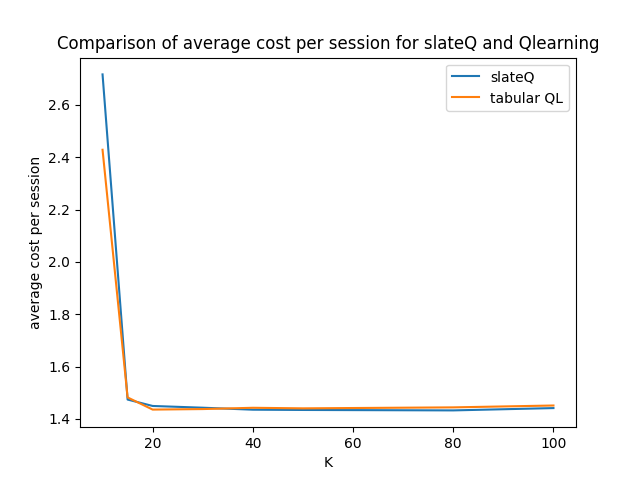
\includegraphics[width=0.48\linewidth]{Figure_1.png}
        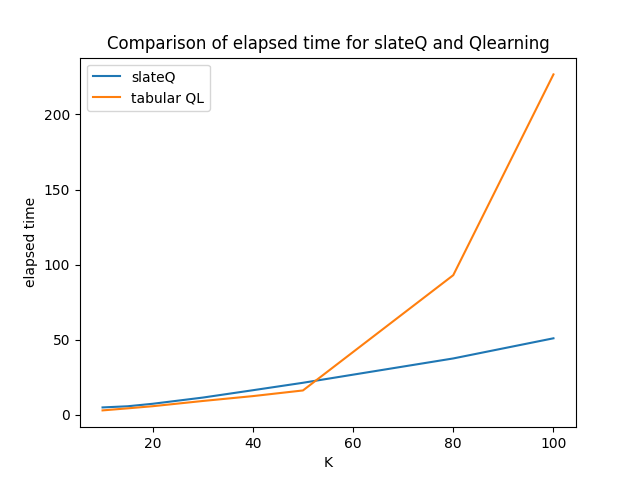
\includegraphics[width=0.48\linewidth]{Figure_2.png}
        \begin{itemize}
            \item Average cost for SlateQ aligns with Q-Learning and converges to $1.44$.
            \item SlateQ time increases linearly with $K$, Q-Learning escalates exponentially.
        \end{itemize}
    \end{frame}
        \begin{frame}{Simulation Results and Analysis}
        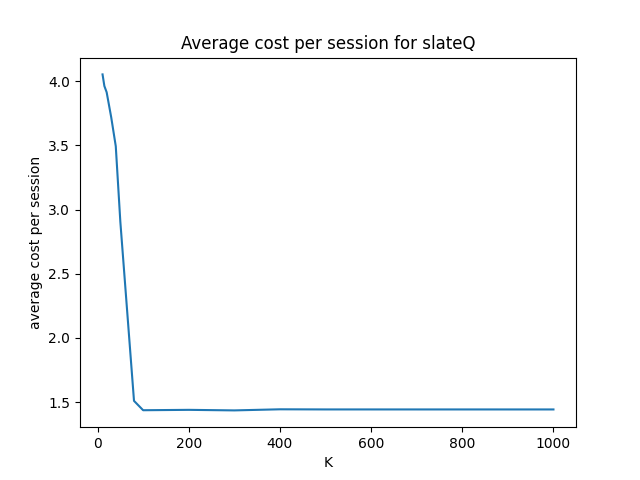
\includegraphics[width=0.48\linewidth]{Figure_3.png}
        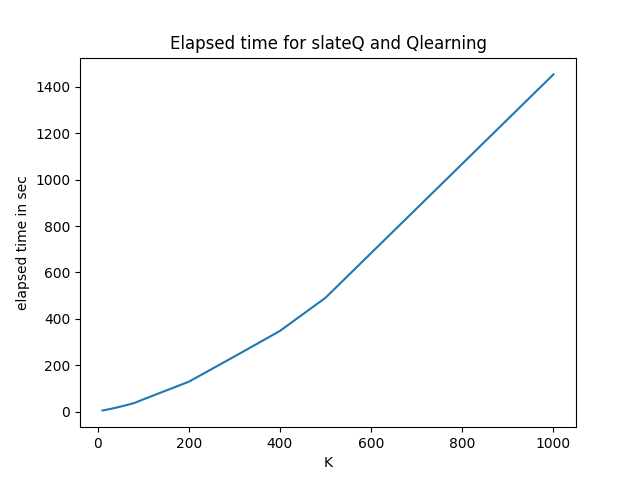
\includegraphics[width=0.48\linewidth]{Figure_4.png}
        \begin{itemize}
            \item With a large library, the algorithm identifies optimal policy, cost remains $1.44$.
            \item Elapsed time exhibits a near-linear increase. Algorithm operates as expected.
        \end{itemize}
        \end{frame}


% Section about the description of the SlateQ algorithm


\end{document}
